%-------------------------------------------------------------------------------
% $HeadURL: http://hb9etc.ch/svn/pluess/tex/da_doku/adaptfilt.tex $
% $Revision: 861 $
% $Author: tobias $
% $Date: 2013-12-23 21:15:48 +0100 (Mon, 23 Dec 2013) $
%-------------------------------------------------------------------------------

\chapter{Physikalischer Hintergrund} 

Blabla \dots

\section{Beschleunigung} 
Dieser Abschnitt basiert auf dem Unterrichtsskript des Physikunterrichts an der Hochschule 
Luzern \cite{Mechanik}. 
 
Der Ortsvektor $\vec{s}$, die Geschwindigkeit $\vec{v}$ und die Beschleunigung $\vec{a}$ sind
Vektoren, welche einen geometrischen Zusammenhang haben. So ist die Geschwindigkeit die Weg- 
Zuwachs-Rate dadurch die Steigung an die Weg-Zeit-Kurve. 
\begin{equation}
\vec{v}=\frac{d\vec{s}}{dt}
\end{equation}
Die Beschleunigung ist die Geschwindigkeits-Zuwachs-Rate und somit die Steigung an die 
Geschwin-digkeit-Zeit-Kurve. 
\begin{equation}
\vec{a}=\frac{d\vec{v}}{dt}=\frac{d^2\vec{s}}{dt}
\end{equation}
Eine weitere Ableitung f�hrt zum Ruck. Die Ableitungen k�nnen beliebig weitergef�hrt werden. 
Umgekehrt kann die Geschwindigkeit oder die zur�ckgelegte Strecke durch Integration der 
Beschleunigung bzw. Geschwindigkeit berechnet werden. 

Bei der Bahnkurve zeigt der Geschwindigkeitsvektor immer tangential zur Bahnkurve. Der
Beschleunigungsvektor zeigt immer nach innen. Bei einer Kreisf�rmigen Kreisbewegung
zeit der Beschleunigungsvektor zur Mitte des Kreises hin. Diese Beschleunigung nennt
sich Zentripetalbeschleunigung und berechnet sich zu 
\begin{equation}
a_{ZP}=\frac{v^2}{r}= \omega^2\cdot r 
\end{equation} 
mit $v$ der momentanen Geschwindigkeit und $r$ dem Radius des Kreises. 
\newpage
\section{Impuls und Kraftstoss}
Die Beschreibung, wie sich K�rper bewegen, wird mit den drei Axiomen von Newton 
erweitert. Dabei wird die Frage beantwortet, warum sich etwas bewegt. Ein 
K�rper �ndert seine Geschwindigkeit (Beschleunigung) unter Einwirkung einer
Kraft. Dies widerspiegelt sich in der Bewegungsgleichung (zweites Axiom)
\begin{equation}
\vec{F}=m\cdot \vec{a}.
\end{equation}
Eine weitere Beschreibung der Bewegung eines K�rpers ist der Impuls. Er ist das 
Produkt von Masse und Geschwindigkeit. 
\begin{equation}
\vec{p}=m\cdot\vec{v} 
\end{equation}
Das erweiterte Newtonsche Gesetz lautet somit
\begin{equation}
\vec{F}=m\cdot \vec{a} = m\frac{d\vec{v}}{dt}=\frac{d\vec{p}}{dt}
\end{equation}
und l�sst nun auch ver�nderbare Massen zu. Der Kraftstoss $\vec{J}$ ist 
die Fl�che unter der Kraft-Zeit-Kurve. Er entspricht der Impuls�bertragung. 
\begin{equation}
\vec{J} = \int_{t_1}^{t_2} \! \vec{F}(t) \, \mathrm{d}t = \vec{p}_2 - \vec{p}_1
\end{equation}
Aus dem Kraftstoss l�sst sich eine durchschnittlich wirkende Kraft berechnen (\autoref{fig:druchschnittskraft})
\begin{equation}
\vec{F}_{average} = \frac{\vec{J}}{\Delta t} = \frac{\vec{p}_2 - \vec{p}_1}{t_2- t_1} . 
\end{equation}
	\begin{figure}
		\centering
		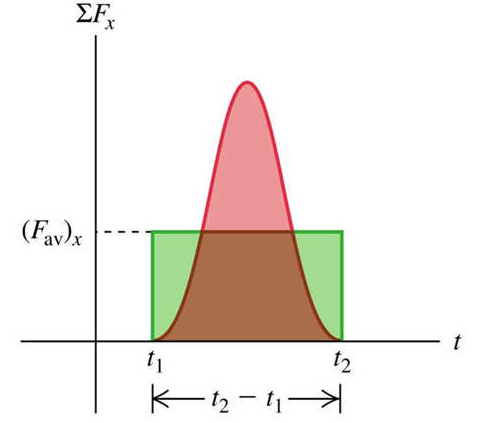
\includegraphics[width=5.5cm]{img/durchschnittskraft.png}
		\caption[Durchschnittliche Kraft $F_{av}$]{Durchschnittliche Kraft $F_{av}$ \cite{Mechanik}}
		\label{fig:druchschnittskraft}
	\end{figure}
Ein Impuls�bertrag kann bei kurzen, heftigen St�ssen oder langen, sanften St�ssen 
gleich gross sein. Die Form des Impulses h�ngt von der Steifigkeit der Materialien ab, welche
aufeinander treffen. Ein steiferes Material erzeugt einen schmaleren Impuls. Die durchschnittliche 
Kraft $F_av$ wird dadurch gr�sser. Das Energiedichtespektrum wird umso breiter, je schmaler der 
Impuls ist. Diese Zusammenh�nge zeigt die \autoref{fig:kraftstoss}.
	\begin{figure}
		\centering
		\captionsetup{width=10cm}
		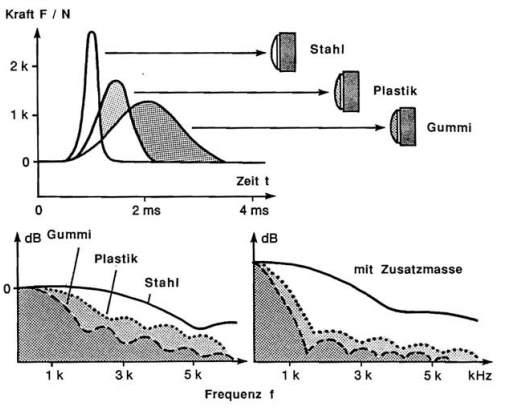
\includegraphics[width=10cm]{img/kraftstoss.png}
		\caption[Kraftstoss]{Die Form des Impulses h�ngt von der Steifigkeit des Materials ab. 
			Je steifer ein Material, desto schmaler der Impuls. Daraus folgt, dass das Energiedichtespektrum
			breiter wird \cite{Ruhm}.}
		\label{fig:kraftstoss}
	\end{figure}


%\section{Mechanische Schwingungen}
%
%\section{Elektromechanische Analogie}

\newpage
\section{Sog-Druckwellen eines Zuges}
	Ein vorbeifahrender Zug erzeugt ein Sog-Druck Feld. Dieses ist in der \autoref{fig:SogDruckFeld}
	dargestellt. Die roten Wellen bezeichnen den �berdruck, die blauen Wellen den Unterdruck. Das
	Sog-Druck Feld ist mit dem Zug verbunden und bewegt sich mit der gleichen Geschwindigkeit voran.
	Das Druckfeld nimmt mit der Zuggeschwindigkeit im Quadrat zu. Es ist umso kleiner, je gr�sser der
	Abstand vom Messpunkt zum Zug ist \cite{Niemann}.
	
	\begin{figure}
		\centering
		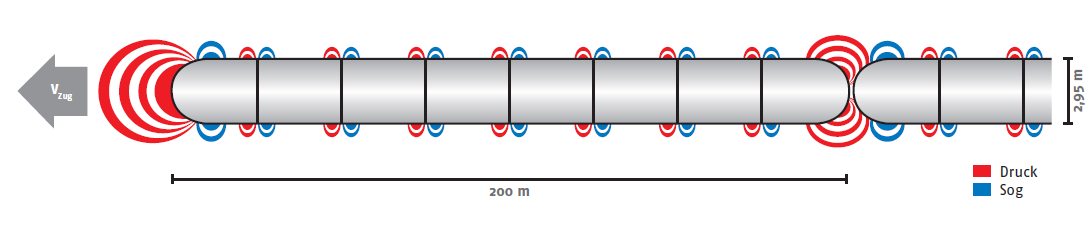
\includegraphics[width=15cm]{img/ZugDruckwelle.png}
		\caption[Typische Druck-Sog-Welle um einen Zug]{Typische Druck-Sog-Welle um einen Zug mit Geschwindigkeit $v_{Zug}$ aus \cite{Niemann}}
		\label{fig:SogDruckFeld}
	\end{figure}	
	Ein typischer Druckverlauf bei einem vorbeifahrenden Zug ist in der \autoref{fig:verlaufDruckwelle}
	gezeigt. Bei der Anfahrt des Zuges wird ein Druck-Sogwechsel gemessen, bei der Ausfahrt der Zuges
	einen Sog-Druckwechsel. Dort entstehen die gr�ssten Druckdifferenzen. Ebenfalls grosse
	Druckdifferenzen k�nnen bei den Kupplungsstellen der Zugzeile gemessen werden \cite{Niemann}.
	\begin{SCfigure}
		\centering
		\vspace{-0.5cm}
		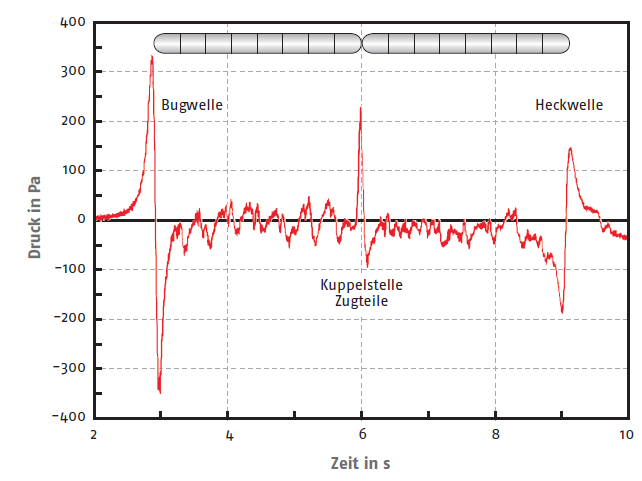
\includegraphics[width=8cm]{img/VerlaufDruckwelleZug.png}
		\caption[Typische Druck-Sog-Welle um einen Zug]{Typischer Druckverlauf bei einem vorbeifahrenden Zug aus \cite{Niemann}}
		\label{fig:verlaufDruckwelle}
	\end{SCfigure}
	Der Abstand zwischen Durck- und Sogwelle L h�ngt nich von der Zugsgeschwindigkeit $v_{Zug}$ ab,
	jedoch vom Wandabstand zur Gleisachse $a_g$. 
	\newpage
	Der Zusammenhang zwischen Wandabstand $a_g$ und Abstand L wurde von Niemann et. Al \cite{Niemann} hergeleitet: 
	\begin{equation}
	L=6.9 \cdot (\frac{a_g}{3.8})^{0.65} 
	\end{equation}
	Bei zugnahen W�nden wird von L=6.9m ausgegangen. 
	Der zeitliche Abstand ist von $v_{Zug}$ abh�ngig und betr�gt bei zugnahen W�nden und der maximalen 
	Durchfahrtsgeschwindigkeit an Bahnh�fen von 200km/h 12ms. Je gr�sser der Wandabstand, desto gr�sser der Abstand 
	zwischen Durck- und Sogwelle und desto l�nger wird auch der zeitliche Abstand.  